\documentclass[]{book}
\usepackage{lmodern}
\usepackage{amssymb,amsmath}
\usepackage{ifxetex,ifluatex}
\usepackage{fixltx2e} % provides \textsubscript
\ifnum 0\ifxetex 1\fi\ifluatex 1\fi=0 % if pdftex
  \usepackage[T1]{fontenc}
  \usepackage[utf8]{inputenc}
\else % if luatex or xelatex
  \ifxetex
    \usepackage{mathspec}
  \else
    \usepackage{fontspec}
  \fi
  \defaultfontfeatures{Ligatures=TeX,Scale=MatchLowercase}
\fi
% use upquote if available, for straight quotes in verbatim environments
\IfFileExists{upquote.sty}{\usepackage{upquote}}{}
% use microtype if available
\IfFileExists{microtype.sty}{%
\usepackage{microtype}
\UseMicrotypeSet[protrusion]{basicmath} % disable protrusion for tt fonts
}{}
\usepackage[margin=1in]{geometry}
\usepackage{hyperref}
\hypersetup{unicode=true,
            pdftitle={Ciencia de Datos para Gente Sociable},
            pdfauthor={Antonio Vazquez Brust},
            pdfborder={0 0 0},
            breaklinks=true}
\urlstyle{same}  % don't use monospace font for urls
\usepackage{natbib}
\bibliographystyle{apalike}
\usepackage{color}
\usepackage{fancyvrb}
\newcommand{\VerbBar}{|}
\newcommand{\VERB}{\Verb[commandchars=\\\{\}]}
\DefineVerbatimEnvironment{Highlighting}{Verbatim}{commandchars=\\\{\}}
% Add ',fontsize=\small' for more characters per line
\usepackage{framed}
\definecolor{shadecolor}{RGB}{248,248,248}
\newenvironment{Shaded}{\begin{snugshade}}{\end{snugshade}}
\newcommand{\KeywordTok}[1]{\textcolor[rgb]{0.13,0.29,0.53}{\textbf{#1}}}
\newcommand{\DataTypeTok}[1]{\textcolor[rgb]{0.13,0.29,0.53}{#1}}
\newcommand{\DecValTok}[1]{\textcolor[rgb]{0.00,0.00,0.81}{#1}}
\newcommand{\BaseNTok}[1]{\textcolor[rgb]{0.00,0.00,0.81}{#1}}
\newcommand{\FloatTok}[1]{\textcolor[rgb]{0.00,0.00,0.81}{#1}}
\newcommand{\ConstantTok}[1]{\textcolor[rgb]{0.00,0.00,0.00}{#1}}
\newcommand{\CharTok}[1]{\textcolor[rgb]{0.31,0.60,0.02}{#1}}
\newcommand{\SpecialCharTok}[1]{\textcolor[rgb]{0.00,0.00,0.00}{#1}}
\newcommand{\StringTok}[1]{\textcolor[rgb]{0.31,0.60,0.02}{#1}}
\newcommand{\VerbatimStringTok}[1]{\textcolor[rgb]{0.31,0.60,0.02}{#1}}
\newcommand{\SpecialStringTok}[1]{\textcolor[rgb]{0.31,0.60,0.02}{#1}}
\newcommand{\ImportTok}[1]{#1}
\newcommand{\CommentTok}[1]{\textcolor[rgb]{0.56,0.35,0.01}{\textit{#1}}}
\newcommand{\DocumentationTok}[1]{\textcolor[rgb]{0.56,0.35,0.01}{\textbf{\textit{#1}}}}
\newcommand{\AnnotationTok}[1]{\textcolor[rgb]{0.56,0.35,0.01}{\textbf{\textit{#1}}}}
\newcommand{\CommentVarTok}[1]{\textcolor[rgb]{0.56,0.35,0.01}{\textbf{\textit{#1}}}}
\newcommand{\OtherTok}[1]{\textcolor[rgb]{0.56,0.35,0.01}{#1}}
\newcommand{\FunctionTok}[1]{\textcolor[rgb]{0.00,0.00,0.00}{#1}}
\newcommand{\VariableTok}[1]{\textcolor[rgb]{0.00,0.00,0.00}{#1}}
\newcommand{\ControlFlowTok}[1]{\textcolor[rgb]{0.13,0.29,0.53}{\textbf{#1}}}
\newcommand{\OperatorTok}[1]{\textcolor[rgb]{0.81,0.36,0.00}{\textbf{#1}}}
\newcommand{\BuiltInTok}[1]{#1}
\newcommand{\ExtensionTok}[1]{#1}
\newcommand{\PreprocessorTok}[1]{\textcolor[rgb]{0.56,0.35,0.01}{\textit{#1}}}
\newcommand{\AttributeTok}[1]{\textcolor[rgb]{0.77,0.63,0.00}{#1}}
\newcommand{\RegionMarkerTok}[1]{#1}
\newcommand{\InformationTok}[1]{\textcolor[rgb]{0.56,0.35,0.01}{\textbf{\textit{#1}}}}
\newcommand{\WarningTok}[1]{\textcolor[rgb]{0.56,0.35,0.01}{\textbf{\textit{#1}}}}
\newcommand{\AlertTok}[1]{\textcolor[rgb]{0.94,0.16,0.16}{#1}}
\newcommand{\ErrorTok}[1]{\textcolor[rgb]{0.64,0.00,0.00}{\textbf{#1}}}
\newcommand{\NormalTok}[1]{#1}
\usepackage{longtable,booktabs}
\usepackage{graphicx,grffile}
\makeatletter
\def\maxwidth{\ifdim\Gin@nat@width>\linewidth\linewidth\else\Gin@nat@width\fi}
\def\maxheight{\ifdim\Gin@nat@height>\textheight\textheight\else\Gin@nat@height\fi}
\makeatother
% Scale images if necessary, so that they will not overflow the page
% margins by default, and it is still possible to overwrite the defaults
% using explicit options in \includegraphics[width, height, ...]{}
\setkeys{Gin}{width=\maxwidth,height=\maxheight,keepaspectratio}
\IfFileExists{parskip.sty}{%
\usepackage{parskip}
}{% else
\setlength{\parindent}{0pt}
\setlength{\parskip}{6pt plus 2pt minus 1pt}
}
\setlength{\emergencystretch}{3em}  % prevent overfull lines
\providecommand{\tightlist}{%
  \setlength{\itemsep}{0pt}\setlength{\parskip}{0pt}}
\setcounter{secnumdepth}{5}
% Redefines (sub)paragraphs to behave more like sections
\ifx\paragraph\undefined\else
\let\oldparagraph\paragraph
\renewcommand{\paragraph}[1]{\oldparagraph{#1}\mbox{}}
\fi
\ifx\subparagraph\undefined\else
\let\oldsubparagraph\subparagraph
\renewcommand{\subparagraph}[1]{\oldsubparagraph{#1}\mbox{}}
\fi

%%% Use protect on footnotes to avoid problems with footnotes in titles
\let\rmarkdownfootnote\footnote%
\def\footnote{\protect\rmarkdownfootnote}

%%% Change title format to be more compact
\usepackage{titling}

% Create subtitle command for use in maketitle
\newcommand{\subtitle}[1]{
  \posttitle{
    \begin{center}\large#1\end{center}
    }
}

\setlength{\droptitle}{-2em}
  \title{Ciencia de Datos para Gente Sociable}
  \pretitle{\vspace{\droptitle}\centering\huge}
  \posttitle{\par}
\subtitle{Una introducción a la exploración, análisis y visualización de datos}
  \author{Antonio Vazquez Brust}
  \preauthor{\centering\large\emph}
  \postauthor{\par}
  \predate{\centering\large\emph}
  \postdate{\par}
  \date{2018-01-17}

\usepackage{booktabs}

\usepackage{amsthm}
\newtheorem{theorem}{Theorem}[chapter]
\newtheorem{lemma}{Lemma}[chapter]
\theoremstyle{definition}
\newtheorem{definition}{Definition}[chapter]
\newtheorem{corollary}{Corollary}[chapter]
\newtheorem{proposition}{Proposition}[chapter]
\theoremstyle{definition}
\newtheorem{example}{Example}[chapter]
\theoremstyle{definition}
\newtheorem{exercise}{Exercise}[chapter]
\theoremstyle{remark}
\newtheorem*{remark}{Remark}
\newtheorem*{solution}{Solution}
\begin{document}
\maketitle

{
\setcounter{tocdepth}{1}
\tableofcontents
}
\chapter*{Antes de empezar}\label{antes-de-empezar}
\addcontentsline{toc}{chapter}{Antes de empezar}

\chapter{Una presentación a toda marcha de
R}\label{una-presentacion-a-toda-marcha-de-r}

\texttt{R} es un lenguaje de programación especializado en análisis y
visualización de datos. Es un producto de código abierto, lo cual
significa que cualquier persona puede usarlo y modificarlo sin pagar
licencias ni costos de adquisición de ningún tipo.

Expertos de todo el mundo colaboran en forma activa con el proyecto, no
sólo desarrollando el lenguaje en sí (llamado ``R base''), sino también
extendiéndolo con nuevas habilidades que pueden ser incorporadas por los
usuarios finales en forma de ``paquetes'' de funciones que pueden ser
instaladas.

La calidad del lenguaje en sí, de los paquetes instalables que le
agregan un sinfin de funciones (desde algoritmos de inteligencia
artificial hasta la generación de mapas interactivos) y de la comunidad
de usuarios que comparte información en foros y blogs, ha hecho de R uno
de los lenguajes de pogramación más populares del mundo. En el campo del
análisis de datos, es la herramienta por excelencia en muchas
universidades, empresas de tecnología, y redacciones de periodismo de
datos.

\section{R en acción}\label{r-en-accion}

Vamos a recorrer un ejemplo de lo que somos capaces de hacer cuando
manejamos con soltura una herramienta de análisis como R. Que nadie se
preocupe si algunas de las operaciones parecen no tener sentido, o
resultan arbitrarias. ¡Es normal! Nadie aprende un lenguaje en 10
minutos, sea R o esperanto. La idea es tener exposición temprana a un
caso de uso interesante, usando datos reales. Y que nos sirva como
motivación para practicar luego ejercicios básicos que son muy
necesarios pero, a veces, no tan emocionantes.

\subsection{Crear un proyecto en
RStudio}\label{crear-un-proyecto-en-rstudio}

El primer paso es ejecutar RStudio, que ya deberíamos tener disponible
en nuestro sistema. Una vez abierta la interfaz gráfica, creamos un
proyecto nuevo, cliqueando en
\texttt{"File"\ -\textgreater{}\ "New\ Project..."\ -\textgreater{}\ "New\ Directory"\ -\textgreater{}\ \ "New\ Project"}.
En la ventana que surge, elegir un nombe para el proyecto (por ejemplo)

\begin{Shaded}
\begin{Highlighting}[]
\KeywordTok{library}\NormalTok{(tidyverse)}
\end{Highlighting}
\end{Shaded}

\begin{Shaded}
\begin{Highlighting}[]
\NormalTok{mortalidad <-}\StringTok{ }\KeywordTok{read.csv}\NormalTok{(}\StringTok{'data/mortalidad_infantil_caba.csv'}\NormalTok{)}

\NormalTok{mortalidad}
\end{Highlighting}
\end{Shaded}

\begin{verbatim}
##    Comuna X2010 X2011 X2012 X2013 X2014 X2015 X2016
## 1       1   9.9   9.1  10.7   8.9   4.9   7.6   9.5
## 2       2   6.7   6.6   5.1   7.5   9.2   4.5   3.6
## 3       3   4.9  10.8   7.2  11.9   9.4   5.4   8.0
## 4       4   9.9  11.1  11.8  11.8  12.3   7.2  11.9
## 5       5   3.6   7.2   5.7   8.7   6.7   6.7   8.5
## 6       6   3.2   5.2   9.0   6.8   7.5   5.7   2.4
## 7       7   8.1  11.0   8.9  11.9   8.5   6.4   8.5
## 8       8   7.9   9.7  10.8  10.9  12.7   8.2   9.7
## 9       9   8.1  10.4   8.8   9.3   6.5   6.5  10.1
## 10     10   7.5   7.1   7.3  12.2   5.3   5.8   3.6
## 11     11   5.4   6.3   4.0   5.6   5.3   5.0   6.2
## 12     12   6.5   5.5   5.8   8.0   3.4   3.1   7.1
## 13     13   2.3   7.2   6.2   2.7   6.9   4.7   4.5
## 14     14   6.9   5.0   6.9   5.3   6.8   5.6   3.2
## 15     15   5.4  10.4   7.2   7.2   7.8   4.3   6.4
\end{verbatim}

\begin{Shaded}
\begin{Highlighting}[]
\NormalTok{mortalidad <-}\StringTok{ }\NormalTok{mortalidad }\OperatorTok\StringTok{ }\KeywordTok{gather}\NormalTok{(}\StringTok{"año"}\NormalTok{, mortalidad, X2010}\OperatorTok{:}\NormalTok{X2016)}

\NormalTok{mortalidad}
\end{Highlighting}
\end{Shaded}

\begin{verbatim}
##     Comuna   año mortalidad
## 1        1 X2010        9.9
## 2        2 X2010        6.7
## 3        3 X2010        4.9
## 4        4 X2010        9.9
## 5        5 X2010        3.6
## 6        6 X2010        3.2
## 7        7 X2010        8.1
## 8        8 X2010        7.9
## 9        9 X2010        8.1
## 10      10 X2010        7.5
## 11      11 X2010        5.4
## 12      12 X2010        6.5
## 13      13 X2010        2.3
## 14      14 X2010        6.9
## 15      15 X2010        5.4
## 16       1 X2011        9.1
## 17       2 X2011        6.6
## 18       3 X2011       10.8
## 19       4 X2011       11.1
## 20       5 X2011        7.2
## 21       6 X2011        5.2
## 22       7 X2011       11.0
## 23       8 X2011        9.7
## 24       9 X2011       10.4
## 25      10 X2011        7.1
## 26      11 X2011        6.3
## 27      12 X2011        5.5
## 28      13 X2011        7.2
## 29      14 X2011        5.0
## 30      15 X2011       10.4
## 31       1 X2012       10.7
## 32       2 X2012        5.1
## 33       3 X2012        7.2
## 34       4 X2012       11.8
## 35       5 X2012        5.7
## 36       6 X2012        9.0
## 37       7 X2012        8.9
## 38       8 X2012       10.8
## 39       9 X2012        8.8
## 40      10 X2012        7.3
## 41      11 X2012        4.0
## 42      12 X2012        5.8
## 43      13 X2012        6.2
## 44      14 X2012        6.9
## 45      15 X2012        7.2
## 46       1 X2013        8.9
## 47       2 X2013        7.5
## 48       3 X2013       11.9
## 49       4 X2013       11.8
## 50       5 X2013        8.7
## 51       6 X2013        6.8
## 52       7 X2013       11.9
## 53       8 X2013       10.9
## 54       9 X2013        9.3
## 55      10 X2013       12.2
## 56      11 X2013        5.6
## 57      12 X2013        8.0
## 58      13 X2013        2.7
## 59      14 X2013        5.3
## 60      15 X2013        7.2
## 61       1 X2014        4.9
## 62       2 X2014        9.2
## 63       3 X2014        9.4
## 64       4 X2014       12.3
## 65       5 X2014        6.7
## 66       6 X2014        7.5
## 67       7 X2014        8.5
## 68       8 X2014       12.7
## 69       9 X2014        6.5
## 70      10 X2014        5.3
## 71      11 X2014        5.3
## 72      12 X2014        3.4
## 73      13 X2014        6.9
## 74      14 X2014        6.8
## 75      15 X2014        7.8
## 76       1 X2015        7.6
## 77       2 X2015        4.5
## 78       3 X2015        5.4
## 79       4 X2015        7.2
## 80       5 X2015        6.7
## 81       6 X2015        5.7
## 82       7 X2015        6.4
## 83       8 X2015        8.2
## 84       9 X2015        6.5
## 85      10 X2015        5.8
## 86      11 X2015        5.0
## 87      12 X2015        3.1
## 88      13 X2015        4.7
## 89      14 X2015        5.6
## 90      15 X2015        4.3
## 91       1 X2016        9.5
## 92       2 X2016        3.6
## 93       3 X2016        8.0
## 94       4 X2016       11.9
## 95       5 X2016        8.5
## 96       6 X2016        2.4
## 97       7 X2016        8.5
## 98       8 X2016        9.7
## 99       9 X2016       10.1
## 100     10 X2016        3.6
## 101     11 X2016        6.2
## 102     12 X2016        7.1
## 103     13 X2016        4.5
## 104     14 X2016        3.2
## 105     15 X2016        6.4
\end{verbatim}

\begin{Shaded}
\begin{Highlighting}[]
\NormalTok{mortalidad <-}\StringTok{ }\NormalTok{mortalidad }\OperatorTok\StringTok{ }\KeywordTok{mutate}\NormalTok{(añ}\DataTypeTok{o =} \KeywordTok{sub}\NormalTok{(}\StringTok{'X'}\NormalTok{, }\StringTok{""}\NormalTok{, año),}
\NormalTok{                                    añ}\DataTypeTok{o =} \KeywordTok{as.integer}\NormalTok{(año))}

\NormalTok{mortalidad}
\end{Highlighting}
\end{Shaded}

\begin{verbatim}
##     Comuna  año mortalidad
## 1        1 2010        9.9
## 2        2 2010        6.7
## 3        3 2010        4.9
## 4        4 2010        9.9
## 5        5 2010        3.6
## 6        6 2010        3.2
## 7        7 2010        8.1
## 8        8 2010        7.9
## 9        9 2010        8.1
## 10      10 2010        7.5
## 11      11 2010        5.4
## 12      12 2010        6.5
## 13      13 2010        2.3
## 14      14 2010        6.9
## 15      15 2010        5.4
## 16       1 2011        9.1
## 17       2 2011        6.6
## 18       3 2011       10.8
## 19       4 2011       11.1
## 20       5 2011        7.2
## 21       6 2011        5.2
## 22       7 2011       11.0
## 23       8 2011        9.7
## 24       9 2011       10.4
## 25      10 2011        7.1
## 26      11 2011        6.3
## 27      12 2011        5.5
## 28      13 2011        7.2
## 29      14 2011        5.0
## 30      15 2011       10.4
## 31       1 2012       10.7
## 32       2 2012        5.1
## 33       3 2012        7.2
## 34       4 2012       11.8
## 35       5 2012        5.7
## 36       6 2012        9.0
## 37       7 2012        8.9
## 38       8 2012       10.8
## 39       9 2012        8.8
## 40      10 2012        7.3
## 41      11 2012        4.0
## 42      12 2012        5.8
## 43      13 2012        6.2
## 44      14 2012        6.9
## 45      15 2012        7.2
## 46       1 2013        8.9
## 47       2 2013        7.5
## 48       3 2013       11.9
## 49       4 2013       11.8
## 50       5 2013        8.7
## 51       6 2013        6.8
## 52       7 2013       11.9
## 53       8 2013       10.9
## 54       9 2013        9.3
## 55      10 2013       12.2
## 56      11 2013        5.6
## 57      12 2013        8.0
## 58      13 2013        2.7
## 59      14 2013        5.3
## 60      15 2013        7.2
## 61       1 2014        4.9
## 62       2 2014        9.2
## 63       3 2014        9.4
## 64       4 2014       12.3
## 65       5 2014        6.7
## 66       6 2014        7.5
## 67       7 2014        8.5
## 68       8 2014       12.7
## 69       9 2014        6.5
## 70      10 2014        5.3
## 71      11 2014        5.3
## 72      12 2014        3.4
## 73      13 2014        6.9
## 74      14 2014        6.8
## 75      15 2014        7.8
## 76       1 2015        7.6
## 77       2 2015        4.5
## 78       3 2015        5.4
## 79       4 2015        7.2
## 80       5 2015        6.7
## 81       6 2015        5.7
## 82       7 2015        6.4
## 83       8 2015        8.2
## 84       9 2015        6.5
## 85      10 2015        5.8
## 86      11 2015        5.0
## 87      12 2015        3.1
## 88      13 2015        4.7
## 89      14 2015        5.6
## 90      15 2015        4.3
## 91       1 2016        9.5
## 92       2 2016        3.6
## 93       3 2016        8.0
## 94       4 2016       11.9
## 95       5 2016        8.5
## 96       6 2016        2.4
## 97       7 2016        8.5
## 98       8 2016        9.7
## 99       9 2016       10.1
## 100     10 2016        3.6
## 101     11 2016        6.2
## 102     12 2016        7.1
## 103     13 2016        4.5
## 104     14 2016        3.2
## 105     15 2016        6.4
\end{verbatim}

\begin{Shaded}
\begin{Highlighting}[]
\KeywordTok{ggplot}\NormalTok{(mortalidad) }\OperatorTok{+}\StringTok{ }
\StringTok{    }\KeywordTok{geom_line}\NormalTok{(}\KeywordTok{aes}\NormalTok{(}\DataTypeTok{x =}\NormalTok{ año, }\DataTypeTok{y =}\NormalTok{ mortalidad, }\DataTypeTok{group =}\NormalTok{ Comuna, }\DataTypeTok{color =} \KeywordTok{as.factor}\NormalTok{(Comuna))) }\OperatorTok{+}
\StringTok{    }\KeywordTok{theme_minimal}\NormalTok{()}
\end{Highlighting}
\end{Shaded}

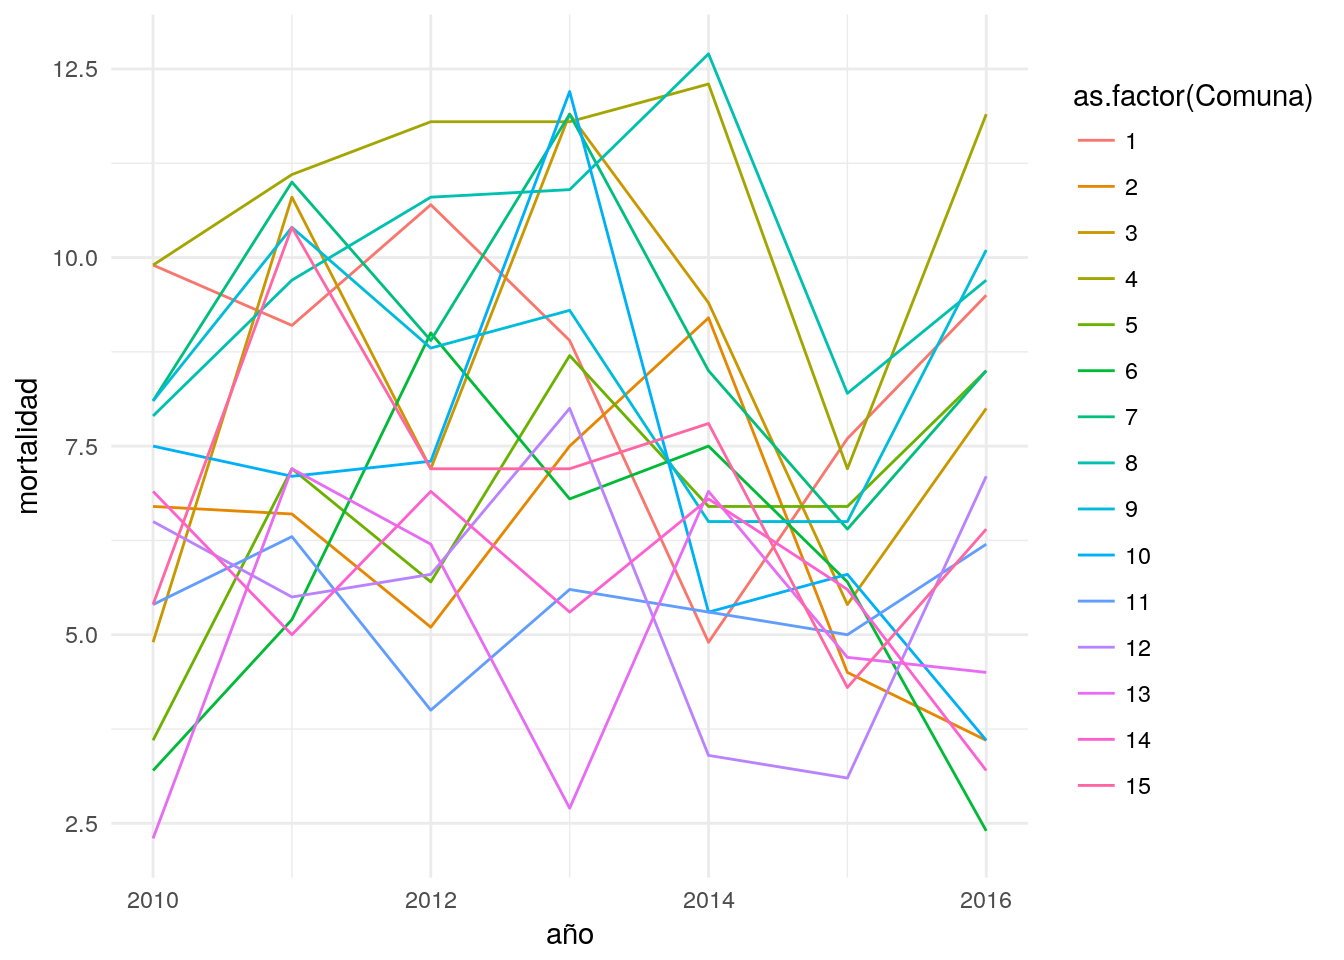
\includegraphics{Ciencia_de_datos_para_gente_sociable_files/figure-latex/unnamed-chunk-2-1.pdf}

\begin{Shaded}
\begin{Highlighting}[]
\KeywordTok{ggplot}\NormalTok{(mortalidad) }\OperatorTok{+}\StringTok{ }
\StringTok{    }\KeywordTok{geom_line}\NormalTok{(}\KeywordTok{aes}\NormalTok{(}\DataTypeTok{x =}\NormalTok{ año, }\DataTypeTok{y =}\NormalTok{ mortalidad, }\DataTypeTok{group =}\NormalTok{ Comuna), }\DataTypeTok{color =} \StringTok{"gray"}\NormalTok{) }\OperatorTok{+}
\StringTok{    }\KeywordTok{geom_line}\NormalTok{(}\DataTypeTok{data =} \KeywordTok{filter}\NormalTok{(mortalidad, Comuna }\OperatorTok{==}\StringTok{ }\DecValTok{4}\NormalTok{), }
              \KeywordTok{aes}\NormalTok{(}\DataTypeTok{x =}\NormalTok{ año, }\DataTypeTok{y =}\NormalTok{ mortalidad, }\DataTypeTok{group =}\NormalTok{ Comuna), }\DataTypeTok{color =} \StringTok{"red"}\NormalTok{) }\OperatorTok{+}
\StringTok{    }\KeywordTok{theme_minimal}\NormalTok{()}
\end{Highlighting}
\end{Shaded}

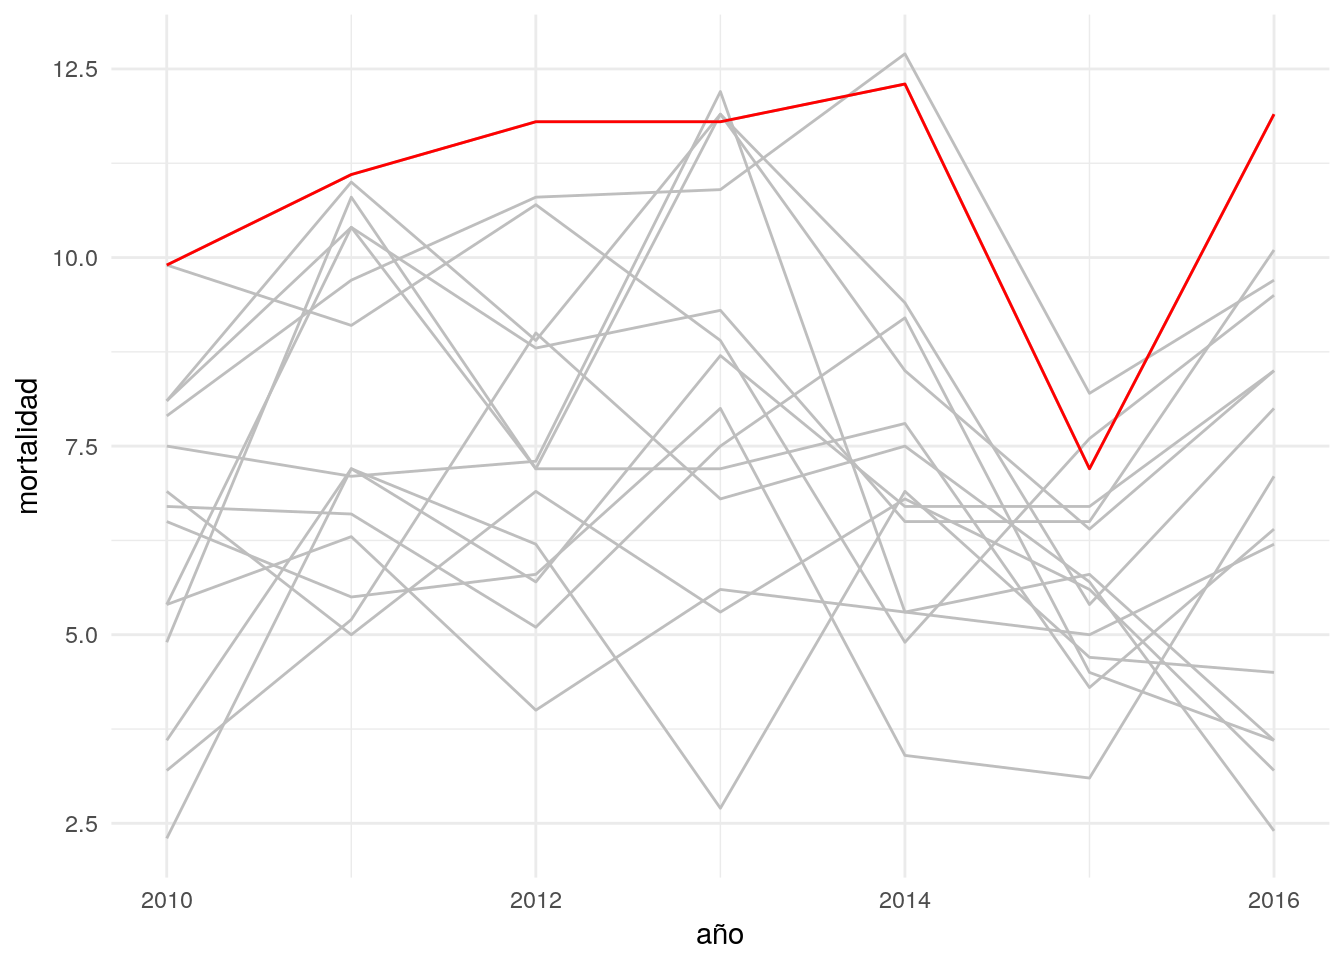
\includegraphics{Ciencia_de_datos_para_gente_sociable_files/figure-latex/unnamed-chunk-2-2.pdf}

\begin{Shaded}
\begin{Highlighting}[]
\KeywordTok{ggplot}\NormalTok{(mortalidad) }\OperatorTok{+}\StringTok{ }
\StringTok{    }\KeywordTok{geom_line}\NormalTok{(}\KeywordTok{aes}\NormalTok{(}\DataTypeTok{x =}\NormalTok{ año, }\DataTypeTok{y =}\NormalTok{ mortalidad, }\DataTypeTok{group =}\NormalTok{ Comuna), }\DataTypeTok{color =} \StringTok{"gray"}\NormalTok{) }\OperatorTok{+}
\StringTok{    }\KeywordTok{geom_line}\NormalTok{(}\DataTypeTok{data =} \KeywordTok{filter}\NormalTok{(mortalidad, Comuna }\OperatorTok{==}\StringTok{ }\DecValTok{4}\NormalTok{), }
              \KeywordTok{aes}\NormalTok{(}\DataTypeTok{x =}\NormalTok{ año, }\DataTypeTok{y =}\NormalTok{ mortalidad, }\DataTypeTok{group =}\NormalTok{ Comuna), }\DataTypeTok{color =} \StringTok{"red"}\NormalTok{) }\OperatorTok{+}
\StringTok{    }\KeywordTok{theme_minimal}\NormalTok{() }\OperatorTok{+}
\StringTok{    }\KeywordTok{labs}\NormalTok{(}\DataTypeTok{title =} \StringTok{"Tasa de mortalidad infantil por comuna"}\NormalTok{, }
         \DataTypeTok{subtitle =} \StringTok{"CABA, 2010 - 206"}\NormalTok{,}
         \DataTypeTok{caption =} \StringTok{"Tasa de la Comuna 4 (barrio de Flores) resaltada"}\NormalTok{)}
\end{Highlighting}
\end{Shaded}

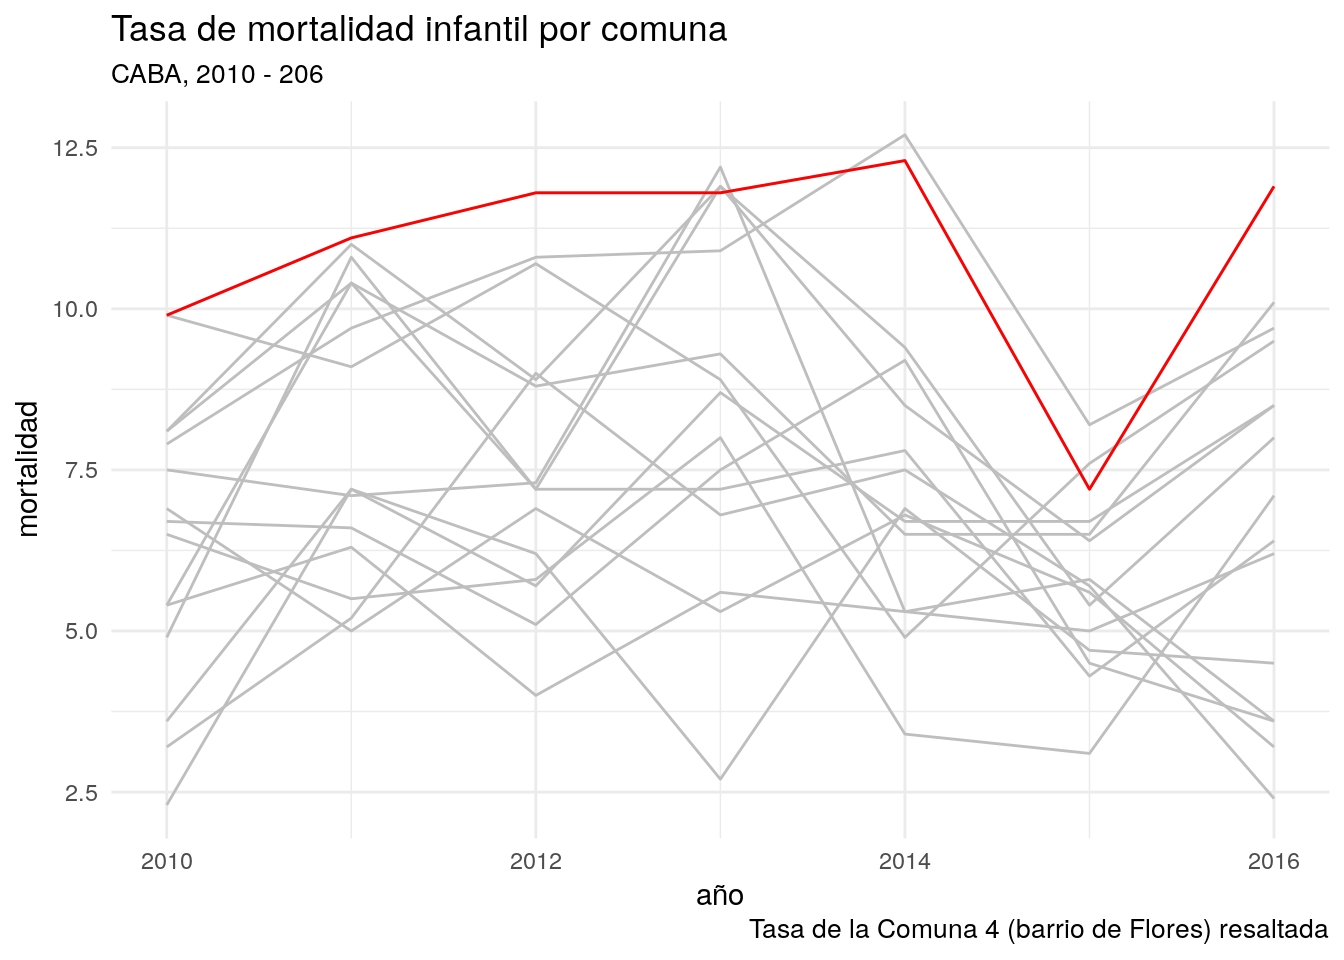
\includegraphics{Ciencia_de_datos_para_gente_sociable_files/figure-latex/unnamed-chunk-2-3.pdf}

\chapter{Literature}\label{literature}

\chapter{Methods}\label{methods}

\chapter{Applications}\label{applications}

\section{Example one}\label{example-one}

\section{Example two}\label{example-two}

\chapter{Final Words}\label{final-words}

\chapter{Placeholder}\label{placeholder}

\bibliography{packages.bib,book.bib}


\end{document}
